\documentclass[a4paper]{article}

%\usepackage[export]{adjustbox}
\usepackage{subcaption}
\usepackage{fullpage}
\usepackage{su18}
\usepackage{cite}


\header{%
  assignment={Protein Sequence analysis using sequential neural networks},%
  authors={Casper Lisager Frandsen <\texttt{fsn483}>,\\
           Marc Pedersen <\texttt{wfj327}>},
  shortAuthors={},%
  date={Github: \url{https://github.com/Cavtheman/proteinbachelor.git}\\ Version 1 \\\textbf{Due:} June 8th}
}

\renewcommand{\thesection}{\arabic{section}.}
\renewcommand{\thesubsection}{(\alph{subsection})}


\begin{document}

\maketitle

\newpage
\tableofcontents
\newpage

\section{Introduction}
% RNN vs CNN
% Protein Representation
%
Proteins encode many different significant and more or less useful properties in the organisms they exist in. Proteins consist of long chains of up to several hundred amino acids, with some of these being more important for the proteins properties than others. Now, how a protein interacts with other proteins is primarily based on their $3$D shape, which is generally called their tertiary structure. A Proteins primary structure consists of the amino acid chain, while their secondary structure is the shape that these chains form. (eg. helices or sheets). The tertiary structure would then describe the way that these are combined and folded in $3$D space. Because their interactions with other proteins are primarily affected by their tertiary structure, finding this is very important for understanding a protein's function. \\

\noindent
Finding a protein's tertiary structure has historically been a very slow and expensive process however, generally requiring significant amounts of lab work and time. On the contrary, finding their primary structures (amino acid sequences) is relatively very easy, and the amount of data available in this form is actually increasing exponentially.\cite{seqcount} This means that there is a significantly larger amount of data available with the primary structure of proteins. Thus, finding a meaningful representation that can be used to say something about other properties of a protein using only the primary structure is an active area of research. There are many parallels between tertiary structure prediction and natural language processing (NLP) in that the data consists of sequences of unknown length containing many long-range dependencies between subsequences with high importance.\\

\noindent
Recurrent Neural Networks (RNNs) in various forms have been go-to architectures for most modelling tasks regarding these types of sequences for a long time now and with good reason. They provide good results and can, given proper architectures, remember many of the dependencies between subsequences and achieve state-of-the-art performance on many protein representation and prediction tasks. However, a recent paper has shown that in many cases, Convolutional Neural Networks (CNNs) can achieve as good, if not better results when applied properly.\cite{intro} We will in this paper reproduce an RNN that can learn some representation from these raw sequences by training it for next-token prediction.\cite{unirep} The idea here is that if the model can accurately predict what the next amino acid is in these long chains, it is because it has learned something inherent in the structure of this protein.\\

\noindent
We will then compare these results to a CNN that is trained to predict each token in the input sequence. This is an easy task, except the input will be changed to something incorrect. In this case, the idea is that the model will end up having to learn what each element is supposed to be from the context around it. We do this by encoding the primary structure of the protein into an arbitrarily small representation, and then decoding this representation to output the same primary structure. Having learned how to do this well must mean that it has also learned something inherent about the structure of these proteins, and thus the encoding of the protein must have some meaningful information about its structure.\\

\noindent
To evaluate the very different results of these models, we will be training a simple linear regression model on each models internal representation of the protein.


\section{Theory}
\subsection{General neural network models}
A neural network is a deep learning technique. Deep learning is a branch of machine learning and is from a mathematical perspective - A method of representing differential functions mapping one type of variable, into another type of variable.

$$
f(In\_variable) = out\_variable
$$

\noindent
Neural networks have high performance in detection and recognizing tasks. Through learning and classifying complex pattern features, it can learn some representation of a given input. The neural network model is inspired by how biological neurons work in the brain. The objective of neural network models is to create a model that is teachable and can perform problem-solving tasks, which is easy for a human, but difficult for a computer.\\

\noindent
As for the brain, a neural network has neurons. These neurons are called nodes. these neurons are clustered in different layers, and each layer of neurons is in some way connected with other neurons in the other layers.  A simple version of a neural network is the feed-forward neural network. in this kind of neural network, there are no connections between the nodes, that creates a cycle. This implies the data travels only in one direction. This kind of architecture is composed of an input layer, 1 or more hidden layers, and an output layer. Given any kind of input variable X, the model creates its estimate of the output\_variable Y, after the input has been processed by the different layers.
In general, if you feed a model $\mathbb{K}$ the input variable $\mathbb{X}$, it will produce the output value $\mathbb{Y}:$

$$
\mathbb{K}: \mathbb{X} \to \mathbb{Y}
$$

\begin{figure}[!ht]
  \centering
  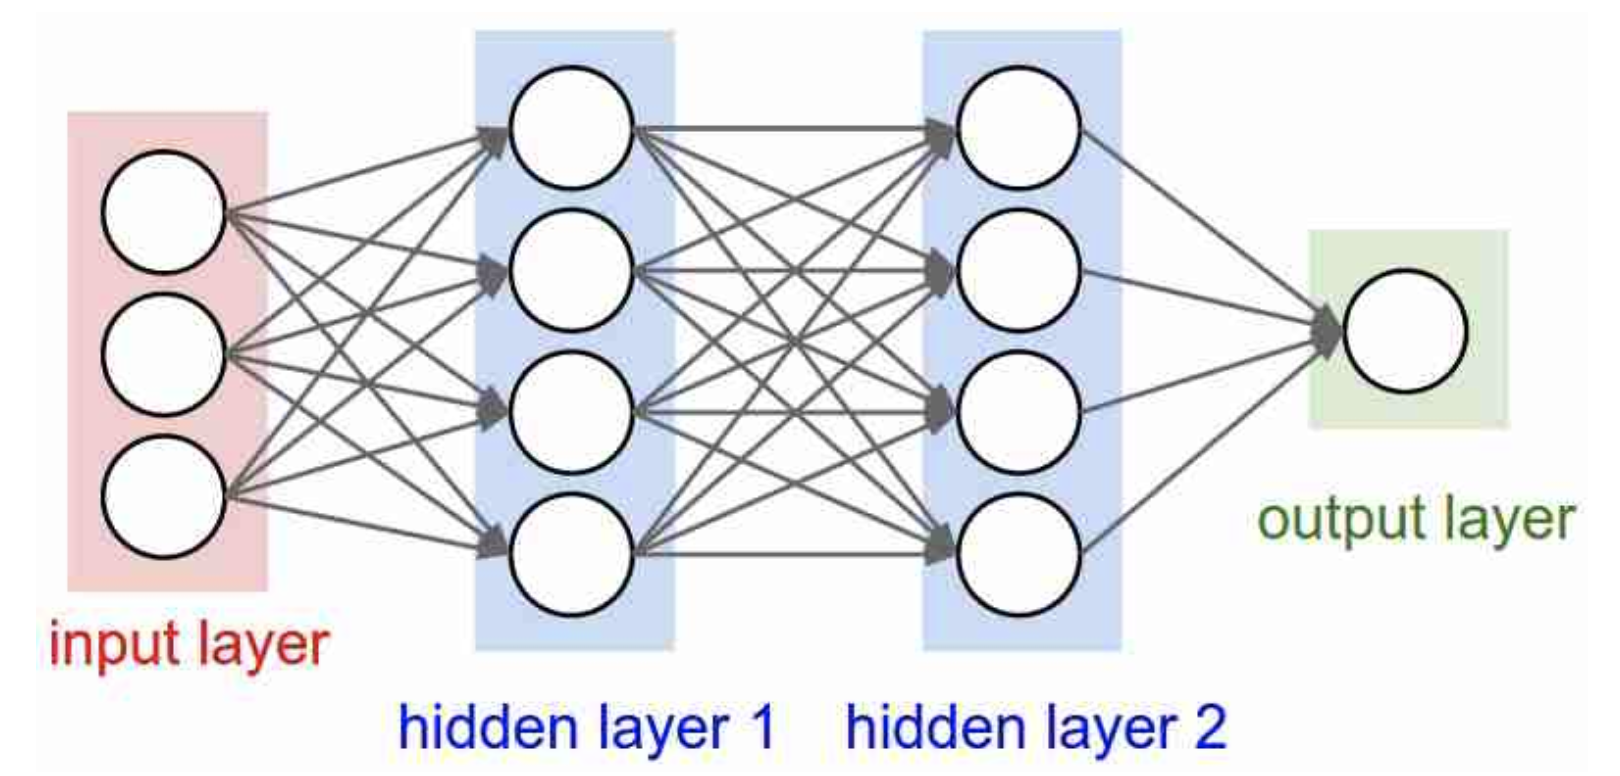
\includegraphics[scale=0.4]{latex/IMGs/NN.png}
  \caption{Feed forward model, with two hidden layers.}\label{Baseline:before}
\end{figure}

\noindent
In our project we use two neural networks, A convulutional neural network and recurrent neural network. These will be explained more in-depth later in report.

\noindent
In machine learning, we have two methods called supervised- and unsupervised learning. Supervised learning is when the data is labeled. The goal is to use some input to predict one or more given labeled outputs. Making the model learn an unknown function, which can map the input to the labeled output. Unsupervised learning is learning without a label. The goal is to learn some useful insight into the data's characteristics, without having a supervising label. In our project, we focused mainly on unsupervised learning, given we had limited labeled data, but a great amount of unlabeled data. \\

\subsection{Hidden layers}

A hidden layers in neural network consists are layers in between the input layer and the ouput layer. each layer consists of columns of neurons, and are connected to neurons in adjacent layers. The connection between the neurons are called weights, and are represented by a real number value. These weights are individual, meaning that two neurons in the same layer, recieving the same input, can have different weights associated to it. A neuron in a hidden layer, takes as input, all of the attached neurons multiplied by their weight, summed including a fixed bias and passed through an activation function to a scalar-output. this activation function is in our case a lineare rectified unit.\\

\noindent
Presenting this as a function, the sum of the multiplied weights and added bias we define as $y_i$. We then define the connected neurons $x_j$ for $j \in$ \{1,...,N\}, where N is the amount of the connected neurons. We define the associated weights as $w_{ij}$ and added bias as $b_i$. Having the activation function as $\phi()$:

\begin{align}
	y_i &= \sum^N_{j=1} x_jw_{ij} + b_i\\
	a_i &= a(y_i) \\
	a_i &=\left\{ \begin{matrix}
		a_i \geq 0 = a_i \\
		\\
		a_i < 0 = 0
	\end{matrix}
	\right.
\end{align}


\begin{figure}[!ht]
  \centering
  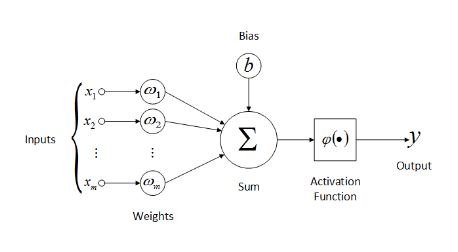
\includegraphics[scale=1.0]{latex/IMGs/neuronFunc.png}
  \caption{Diagram represeinting how a neuron calcutlates its value}\label{Baseline:before}
\end{figure}

\noindent
When training the neural network, the only parameter which is changing is the weights. Since the weight from the neuron(1) is multiplied with the weight connecting to neuron(2), the magnitude of this weight defines how much influence neuron(1) has on neuron(2). Thus, the quality of the model, depends on how good it is at adjusting the weights, and by that learning the model to map input to a nice estimation of a correct output.


\subsection{Convolutional neural network}

\subsubsection{Convolutional neural network}
In our project one of the models, we use is a convolutional neural network(CNN). CNN's are strong tools for classifications of feature maps. In a CNN, the input data goes through one or more layers, where each neuron in each layer is applied with convolutional operations, which are fed to adjacent layers - forming a fully connected neural network layer. \\

\noindent
In our case, each amino acid will be represented as a neuron in the neural network. Since it's a fully connected network, each neurons' value, is calculated by looking at all neurons from the previous layer. This means that each neuron takes the entire sequence as input - applying its weights and then passes it through an activation function. By doing this, the model gets fit to detect important patterns in the sequence.



\subsubsection{Convolutions}
The convolutional layers are what makes CNN's such a strong tool. In general, a convolution consists of a set of learnable filters. Applying a convolutional operation on a neuron is done by using these filters to transform the input in some way, and output the transformed data. As mentioned earlier, CNNs can detect important patterns. The detections of these patterns are happening in these convolutional operations.\\

\noindent
These filters also called 'kernels', are simply just small matrixes initialized with some predefined dimensions and random values. When a kernel is applied on some feature map, the kernel simply convolve across all the feature-channels.\\

\noindent
Having a $M$x$M$ kernel $g$ with stride $1$x$1$, will take the center of the kernel, and stride the kernel over all possible regions of the input, where the kernel can fit. Simply finding the dot-product between the regional values of the input $f$, and the kernel values of $g$.

$$ g = \begin{bmatrix}
1/9 & 1/9 & 1/9 \\
1/9 & 1/9 & 1/9 \\
1/9 & 1/9 & 1/9
\end{bmatrix}
$$

\noindent
This means, that if some were to use, the filter kernel g, on some input feature map. This filter g would simply be a mean filter for the input; averaging all input regions. thus the output features will consist of a matrix with values of all the regions averaged. Using a filter greater than $1$x$1$ will yield a smaller output matrix.

\begin{figure}[!ht]
  \centering
  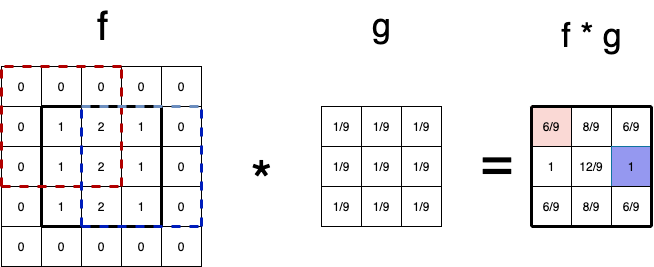
\includegraphics[scale=0.4]{latex/imgs/conv1.png}
  \caption{Shows how a 3x3 mean filter acts on a 5x5 pixel feature map, with stride 1x1}\label{Baseline:before}
\end{figure}

\noindent
Given that we are looking at sequences, which are not two dimensional, but one dimensional, the filtering will look like:

\begin{figure}[!ht]
  \centering
  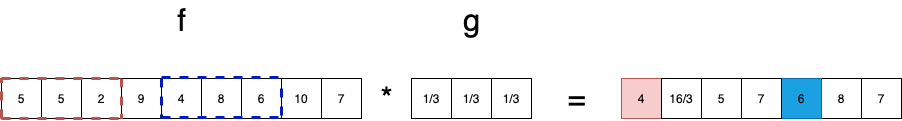
\includegraphics[scale=0.4]{latex/imgs/conv2.png}
  \caption{Shows how a 1x3 mean filter acts on a 1x9 feature map, with stride 1}\label{Baseline:before}
\end{figure}

\noindent
Lastly, the convolutional layers have something called stride. The stride value defines how the filter travels over the input. Meaning how many steps it takes before calculating a new dot-product. In the example given above, we have a stride size of $1$x$1$. This means, that every single region where a $3$x$3$ can fit in the input, the dot-product will be calculated. If we were to change the stride to size $2$x$1$, the output would become smaller, since we take bigger steps, before taking the dot-product.

\begin{figure}[!ht]
  \centering
  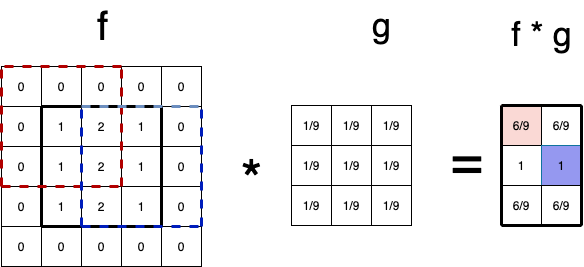
\includegraphics[scale=0.4]{latex/imgs/conv1_stride.png}
  \caption{Shows how a 3x3 mean filter acts on a 5x5 pixel feature map, with stride 2x1}\label{Baseline:before}
\end{figure}

\begin{figure}[!ht]
  \centering
  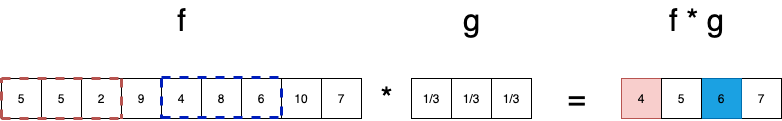
\includegraphics[scale=0.4]{latex/imgs/conv2_stride.png}
  \caption{Shows how a 1x3 mean filter acts on a 1x9 feature map, with stride 2}\label{Baseline:before}
\end{figure}


\subsubsection{Pooling}
Pooling is a way of shrinking the non-channel dimension of some input. The idea of pooling reminds a lot about how convolution works. Pooling also operates with a kernel, sliding over the features. Two popular pooling methods are Max-pooling and Average-pooling. In pooling methods, we have a kernel of some predefined size. This kernel will slide over the features, just like how the filter traveled through the features, during a convolution. \\

\noindent
The output of Max-pooling (figure 7), will always take the maximum value, of the features where the kernel is currently at. The output of Average-pooling (figure 8), will take the average of the features where the kernel is currently at. \\


\begin{figure}[!ht]
  \centering
  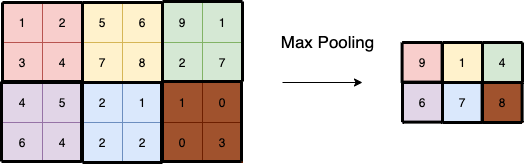
\includegraphics[scale=0.4]{latex/imgs/maxpooling.png}
  \caption{2x2 kernel, max-pool}\label{Baseline:before}
\end{figure}

\noindent
Defining the values within the striding kernel with size $h$x$w$ as $A$, the function looks like:
$$
Maxpool(A) = max(0,A)
$$

\begin{figure}[!ht]
  \centering
  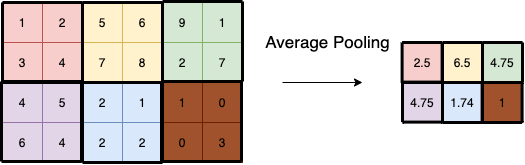
\includegraphics[scale=0.4]{latex/imgs/averagepooling.png}
  \caption{2x2 kernel, average-pool}\label{Baseline:before}
\end{figure}

\noindent
Defining the values within the striding kernel with size $h$x$w$ as $A$, the function looks like:

$$
Averagepool(A) = \frac{\sum_{i \in A} A_i}{h * b}
$$


\subsubsection{Rectified Linear Unit (ReLU)}
The Rectified Linear Unit (RelU) is a very simple activation function, none the less, still a very useful function. When ReLU is called with some input, it will go through all values of the input, turning all negative values to 0, and all positive numbers simply keep their value.

$$
ReLU(input) = max(0,input)
$$
or
\begin{align}
  ReLU(input) &=\left\{
  \begin{matrix}
    input, & \text{ if } input \geq 0\\
    \\
    0,  &\text{ if } input < 0
  \end{matrix}
  \right.
\end{align}

\begin{figure}[!ht]
  \centering
  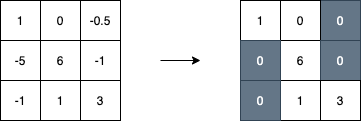
\includegraphics[scale=0.4]{latex/imgs/relu.png}
  \caption{Example of how ReLU() works}\label{Baseline:before}
\end{figure}


\subsubsection{Fully connected layer}
When taking convolutional layers, ReLU layers and pooling layers, stacking them, in way so the output of the first operation becomes the input of the next operation in the stack. When these operations get stacked like this, fully connected layers are often introduced at the end of the last convolution. These fully connected layers are the same as the hidden layers in a feed-forward neural network. In a CNN you can have non-convolutional layers, though at least one is required for it to be a CNN. CNNs can have multiple of these layers. Normally the last hidden layer before the output layer is a convolutional layer since the output of this only shows patterns that a fully connected layer can pick up on, to come up with a specific prediction of a class etc.



\subsection{Recurrent neural network}

\subsubsection{Recurrent neural network}
A Recurrent neural network(RNN), is a neural network model with principle of saving the output, feeding this output as input to the same model. RNNs works with sequences of arbitrary lengths. Sequences are a sets of data having a defined order to it. In our case the sequential data we are working with are the amino acid sequences. RNNs are very good at next token predictions in data.

\noindent
Next token prediction, means predicting the next element in an sequence, given the previous data points have been analyzed.

\begin{figure}[!ht]
  \centering
  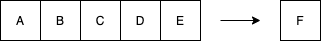
\includegraphics[scale=0.4]{latex/IMGs/AlphabetPred.png}
  \caption{Simple example of how an RNN can predict the next element in the alphabet}\label{Baseline:before}
\end{figure}

\noindent
As for a feed forward neural network, a RNN also has an input layer, hidden layer, and a output layer. Essientially,

\subsubsection{Exploding Gradient}
%Theory behind RNN
%lstm as improvement on rnn
%Theory of lstm, inner workings
%Use of hidden layers
Typical neural networks do not have a state that allows them to "remember" previous data points, for prediction. This is where the basic idea behind a recurrent neural network (RNN for short) comes from. It has a hidden state representing its memory regarding previous data. It will then be able to make decisions regarding new data, taking this previous data into account.

If we take a look at the sentences below, the idea is that the RNN would first be able to understand the nearby context; that the next word is supposed to be a reason for staying home. And also understand the larger context, (that the pandemic is that reason) without needing to remember unnecessary stuff like the words "is", "a" and so on. It should then be able to predict that pandemic would be the next word in the sentence.

\begin{itemize}
	\item There is a pandemic. I had to stay home from university because of the \_\_\_
\end{itemize}

RNNs are extremely flexible in how they can be used. There are, in fact, four main ways they transform the input into something usable. 

The first is in a "one to many" fashion, in which they take a single input and output a sequence. This could be useful for tasks like generating descriptions based on fixed size inputs such as images. 

The second is in a "many to one" fashion in which the input is a sequence, and the network outputs a single result a the end. This is useful in cases where an entire sequence has a single class to be predicted.

The last two both output in a "many to many" fashion, but how they do it is significantly different. The first case outputs a completely new sequence that is not neccesarily the same length as the input sequence, after having seen the entire input. This is useful for networks trying to represent the data in a different way. The last case is the one that will be described further down in this report. This case outputs an element of a new sequence for each element in the input. This means that for each output element, the RNN only knows about previous elements. This makes it the perfect candidate for next token prediction.

\begin{figure}[h]
	\centering
		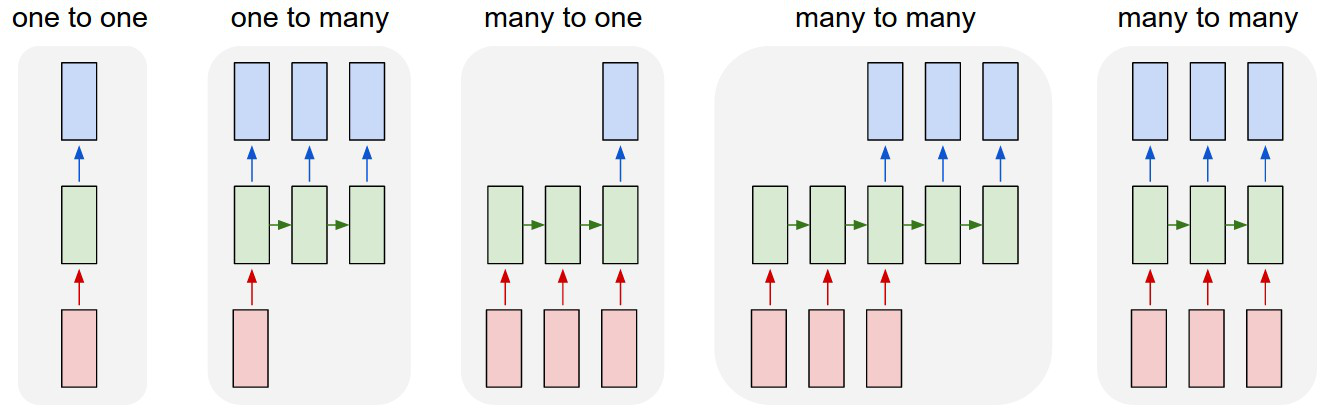
\includegraphics[width=0.5\textwidth]{latex/IMGs/rnn_types.png}}
  	\caption{A visual representation of the output types described. Image Source:\cite{rnn}}
\end{figure}

The basic structure of an RNN is quite simple, consisting of a single linear layer and activation function, which is usually the $tanh$ function. The network is interesting in that each "cell" passes along a hidden state as input to the next cell. This means that each cell takes both the current input element and the previous cell's output and concatenates them and uses this as input to the linear layer.

\begin{figure}[h]
	\centering
		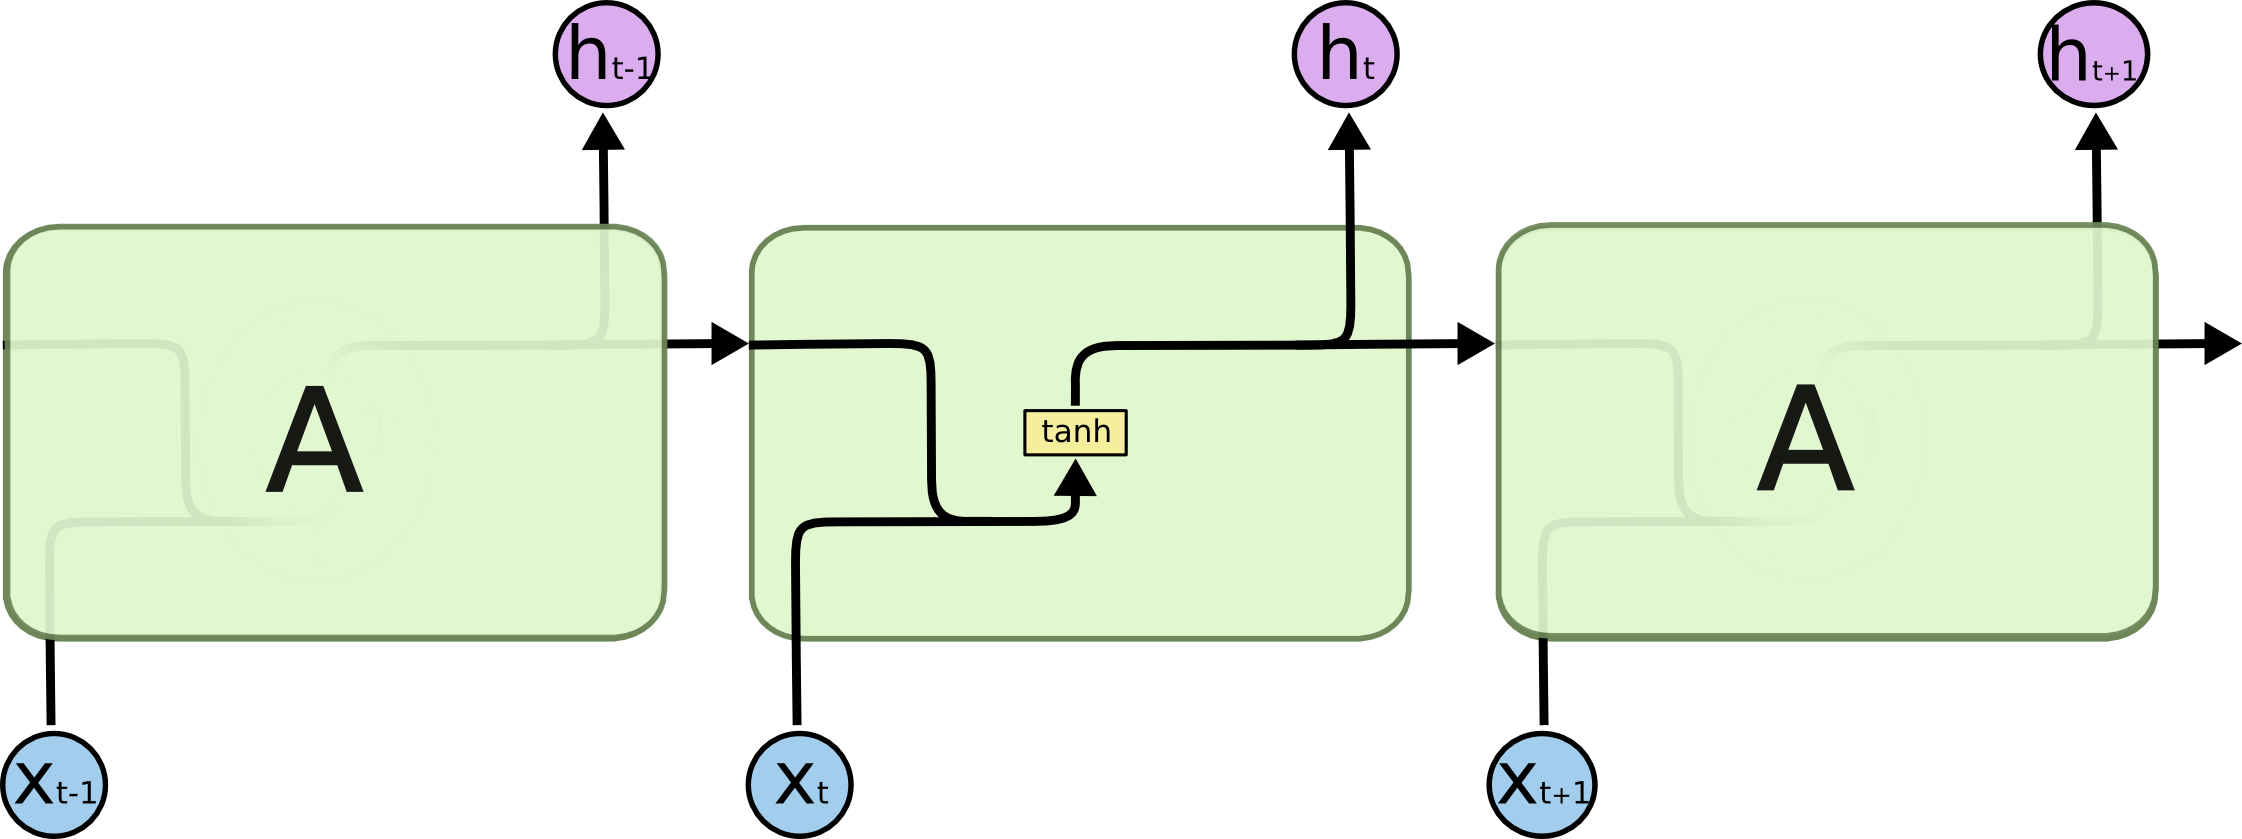
\includegraphics[width=0.5\textwidth]{latex/IMGs/rnn.png}}
  	\caption{A visual representation of the inner structure of an RNN. Image Source:\cite{rnn}}
\end{figure}

\subsubsection{The exploding/vanishing gradient problem}
One major issue with using basic RNNs is the fact that they suffer quite heavily from the exploding/vanishing gradient problem. This problem arises from the fact that very large gradients and gradients very close to zero tend to approach infinity and zero respectively, as they are multiplied together during backpropagation.

To show this, let's consider an RNN network, which for simplicitys sake has a single variable


\subsubsection{LSTM}
\input{latex/rnn/exp_grad}


\subsection{Recurrent Neural Networks}
%Theory behind RNN
%lstm as improvement on rnn
%Theory of lstm, inner workings
%Use of hidden layers
Typical neural networks do not have a state that allows them to "remember" previous data points, for prediction. This is where the basic idea behind a recurrent neural network (RNN for short) comes from. It has a hidden state representing its memory regarding previous data. It will then be able to make decisions regarding new data, taking this previous data into account.

If we take a look at the sentences below, the idea is that the RNN would first be able to understand the nearby context; that the next word is supposed to be a reason for staying home. And also understand the larger context, (that the pandemic is that reason) without needing to remember unnecessary stuff like the words "is", "a" and so on. It should then be able to predict that pandemic would be the next word in the sentence.

\begin{itemize}
	\item There is a pandemic. I had to stay home from university because of the \_\_\_
\end{itemize}

RNNs are extremely flexible in how they can be used. There are, in fact, four main ways they transform the input into something usable. 

The first is in a "one to many" fashion, in which they take a single input and output a sequence. This could be useful for tasks like generating descriptions based on fixed size inputs such as images. 

The second is in a "many to one" fashion in which the input is a sequence, and the network outputs a single result a the end. This is useful in cases where an entire sequence has a single class to be predicted.

The last two both output in a "many to many" fashion, but how they do it is significantly different. The first case outputs a completely new sequence that is not neccesarily the same length as the input sequence, after having seen the entire input. This is useful for networks trying to represent the data in a different way. The last case is the one that will be described further down in this report. This case outputs an element of a new sequence for each element in the input. This means that for each output element, the RNN only knows about previous elements. This makes it the perfect candidate for next token prediction.

\begin{figure}[h]
	\centering
		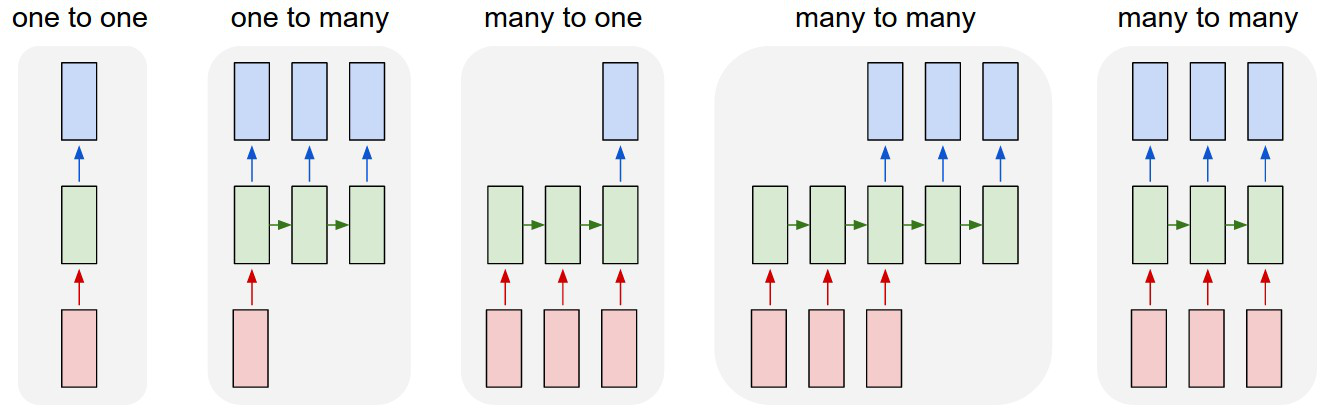
\includegraphics[width=0.5\textwidth]{latex/IMGs/rnn_types.png}}
  	\caption{A visual representation of the output types described. Image Source:\cite{rnn}}
\end{figure}

The basic structure of an RNN is quite simple, consisting of a single linear layer and activation function, which is usually the $tanh$ function. The network is interesting in that each "cell" passes along a hidden state as input to the next cell. This means that each cell takes both the current input element and the previous cell's output and concatenates them and uses this as input to the linear layer.

\begin{figure}[h]
	\centering
		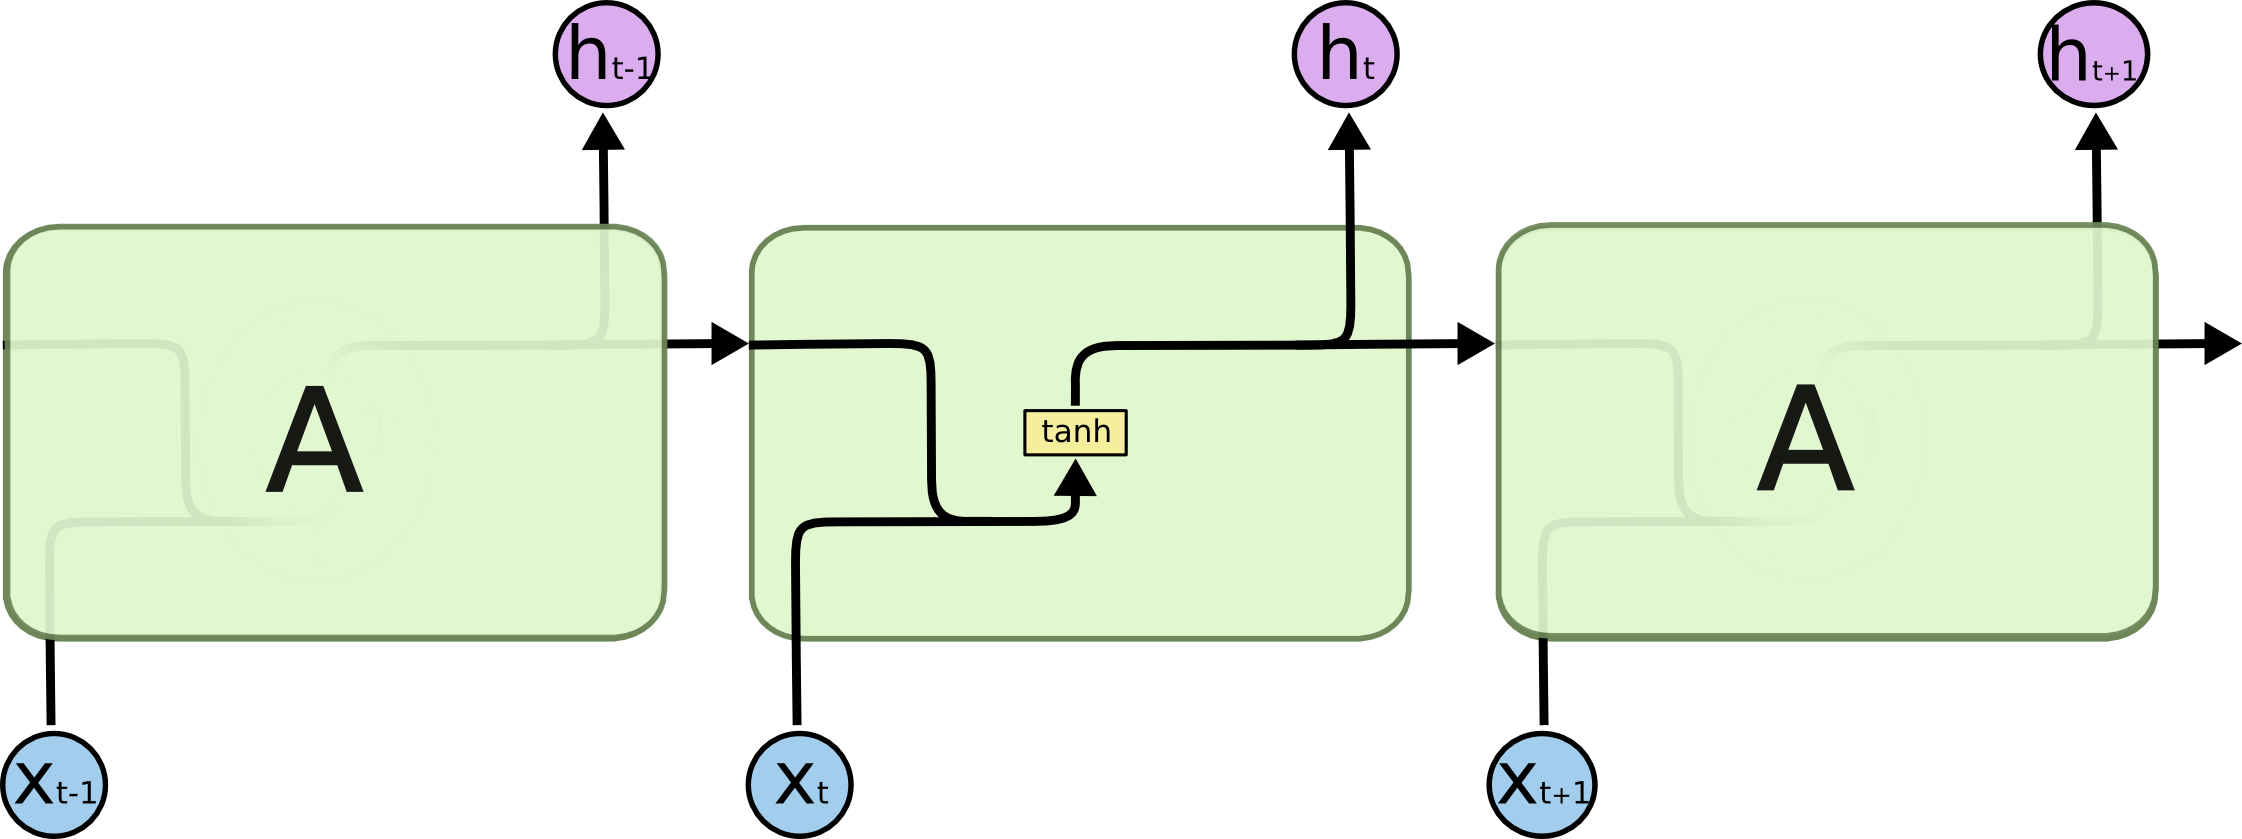
\includegraphics[width=0.5\textwidth]{latex/IMGs/rnn.png}}
  	\caption{A visual representation of the inner structure of an RNN. Image Source:\cite{rnn}}
\end{figure}

\subsubsection{The exploding/vanishing gradient problem}
One major issue with using basic RNNs is the fact that they suffer quite heavily from the exploding/vanishing gradient problem. This problem arises from the fact that very large gradients and gradients very close to zero tend to approach infinity and zero respectively, as they are multiplied together during backpropagation.

To show this, let's consider an RNN network, which for simplicitys sake has a single variable


\subsection{Training the model}
\subsubsection{Training What happens when training}
The goal of training a neural network, is for it to be as effective as possible. Meaning that the predcitions it's making, is as close as the desired output. When training a model, various of different operations and methods are being introduced. \\

\noindent
The training of a neural network, is an iterative process. When a model is being trained, it is fed with some input $x$ tranforming it into an output $\hat{y}$, which is an estimation prediction of the desired value $y$. This prediction is then together with the desired input $y$, fed into an error function; which outputs some cost. An error- or cost function is, a way to estimate the differences between the estimated prediction $\hat{y}$ and $y$, by computing some cost. This cost explains how much $y$ and $\hat{y}$ differentiate from each other.\\

\noindent
Using this cost function, in combination with backpropagation and some optimizer (which we will explain later in the report). It is possible to update, the model's parameters, in a way that minimizes the cost function's output. When the cost value becomes smaller, The amount that $\hat{y}$ deviates from $y$, also becomes smaller. This means that our model, becomes better at predicting a good estimation $\hat{y}$ compared to $y$.



\subsubsection{Error Function}
As mentioned; a loss function describes the differents between $\hat{y}$ and $y$. In our project, we use the Cross-Entropy loss function. To formally understand how this function works, we first have to understand how the 'entropy' part works. \\

\noindent
Given a probability distribution of a set of events where the probabilities sum to 1, the Entropy describes the average information value this distribution has, given the probability of the events happening. This information value is described in bits. Finding the information value for a single occurrence is defined as: $-log_2(p(x))$, where $p(x)$ is the probability of x occurring.\\

\noindent
An example helps formally explaining this: If one was told that tomorrow there will have a 75\% chance of rain and 25\% chance of sun. If that person wakes up the next day, finding out it's not raining, this value this would have a 2-bit information value, because $-log_2(0.25) = 2$ bits. If he woke up the next day seeing it was raining, the value of that information is only 0.41 bits because $-log_2(0.75) = 0.41$ bits. Thus, the higher the probability of the occurrence, the lower the information bit-value will become. The intuition here is that if you are very sure that something is correct, but it isn't, then you learn more than if you were not sure.\\

\noindent
The Entropy function $h$ simply finds the average of the information contained in some occurences $X=\{x_0,x_1,...,x_n\}$ where $\sum^n_{i} p(x_i) = 1$:

\begin{align}
    h(X) = \sum^n_{i=1} p(x_i)(-log_2(p(x_i))) \label{eq:cross_entropy}
\end{align}

\noindent
Using Entropy function from equation ~\ref{eq:cross_entropy} on the weather example, it'll yield $(0.75 * 0.41) + (0.25 * 2) = 0.81$.\\

\noindent
The Cross entropy function $H$ measures the entropy between 2 probability distributions ($P$ and $Q$) over the same set of events. We denote an event from the $P$ distribution as $x_i^{(P)}$ and an event from Q as $x_i^{(Q)}$. Thus, Cross-Entropy function H will look like:

\begin{align}
    H(P,Q) = \frac{1}{n} \sum^n_{i=1} p(x_i^{(P)})(-log_2(p(x_i^{(Q)})))
\end{align}

\noindent
So in our case we want to predict the right amino acids. Say that we are only looking at sequences with 3 different amino acids \{A, C, D\}, and we want to predict the amino acid 'A'. We define the following $y$ and an arbitrary $\hat{y}$.

\begin{table}[h]
\centering
\begin{tabular}{|l|l|l|l|}
\hline
           & $p(A)$ & $p(C)$ & $p(D)$ \\ \hline
$y$       & $1.0$  & $0.0$  & $0.0 $ \\ \hline
$\hat{y}$ & $0.6$  & $0.10$ & $0.30$ \\ \hline
\end{tabular}
\end{table}

\noindent
Using $y$ and $\hat{y}$ distributions in the Cross Entropy model H, the function will yield the following cost:

\begin{align}
    H(y,\hat{y}) = 0.736
\end{align}

\begin{table}[h]
\centering
\begin{tabular}{|l|l|l|l|}
\hline
           & $p(A)$ & $p(C)$ & $p(D)$ \\ \hline
$y$       & $1.0$  & $0.0$  & $0.0 $ \\ \hline
$\hat{y}$ & $0.4$  & $0.30$ & $0.30$ \\ \hline
\end{tabular}
\caption{example of a less confident model}\label{Baseline:before}
\end{table}

\noindent
Using this example of a less confident model, the function will yield the following cost: $H(y,\hat{y}) = 1.321$\\

\begin{table}[h]
\centering
\begin{tabular}{|l|l|l|l|}
\hline
           & $p(A)$ & $p(C)$ & $p(D)$ \\ \hline
$y$       & $1.0$  & $0.0$  & $0.0 $ \\ \hline
$\hat{y}$ & $0.9$  & $0.08$ & $0.02$ \\ \hline
\end{tabular}
\caption{example of a more confident model}\label{Baseline:before}
\end{table}

\noindent
Using this example of a more confident model, the function will yield the following cost: $H(y,\hat{y}) = 0.152$\\

\noindent
Now it's clear to see that the greater the difference of $\hat{y}$ and $y$ is, the greater the loss.

\subsubsection{Backpropagation}
When a model is run on some input, it predicts some output $\hat{y}$, which the model wants to evaluate against the desired value $y$. This evaluation happens, with some error function. This error functions outputs some loss-value which is dependent on how much $\hat{y}$ deviates from $y$. The greater the deviation is, the greater the loss/cost will become.
Based on the size of the loss, the models know with how great magnitude it has to adjust its parameters (weights and biases). The goal is to adjust the parameters, so the predicted output $\hat{y}$, gets as close to the desired output $y$.\\

\noindent
Trying every single combination of weights, in the pursuit of finding the best fitting weights for a specific problem, is a very comprehensive task, even for a computer. This problem is being solved with backpropagation. The idea is to find the minimum value of which the loss function can take. Calculating the gradient is a very effective way of finding this minimum. Finding this minimum can be achieved with various gradient descent algorithms. The gradient describes the slope of the function at a specific point in the graph. Assuming we have a function $f$, the following gradient of this function is $f'$. If $f'$ takes some input x, and $f'(x)$ yields a negative result, it means that the graph currently has a negative slop at this current point. Thus, to get closer to a minimum, we have to increase the value of x. \\

\noindent
But a gradient descent algorithm is an algorithm that finds the minimum given it has a gradient available, it is not the algorithm for finding the gradient. Backpropagation is the method of computing the magnitude each weights gradient has on the final error. The way this is done is by propagating backward through the layers, computing the gradient at each weight. \\

\noindent
Each neuron's value is affected by the previous weights. This means, that the gradient of a single weight in one of the first layers, affects the value of all the following layers. If the gradient of this weight is either negative or positive, it will either affect the output in either a negative or positive way. The magnitude of this gradient, explains how great influence this weight has on the output.
To formally understand what is happening, we will look at a very simple neural network, where each layer contains a single neuron, see figure(13). Explaining this as an equation, we define $a^n$ as the predicted output, $L$ and $C$ as some loss-function and cost respectively, and $y$ as the desired output.

\begin{align}
    a^{n-2}& =& \sigma&(a^{n-3}w^{n-2} + b^{n-2}) \\
    a^{n-1}& =& \sigma&(a^{n-2}w^{n-1} + b^{n-1})\\
    a^n& =& \sigma&(a^{n-1}w^n + b^n)\\
    C& =& L&(a^n, y)
\end{align}

\noindent
by looking at this the above equation, it is clear to see that each weight affects the cost. But to find how much a specific weight ($w^n$) affects the cost, we will have to find the derivative of the cost with respect to $w^n$, which is achieved with the chain rule. For this notation, we define $z$ as being the value of a neuron before the activation function.\\

$$
\frac{\partial C}{\partial w^n} =\frac{\partial z^n}{\partial w^n}\frac{\partial a^n}{\partial z^n}\frac{\partial C}{  \partial a^n}
$$

The same counts for how much impact the bias and the activation of the previous layer, recpectivly has on the Cost:

$$
\frac{\partial C}{\partial b^n} =\frac{\partial z^n}{\partial b^n}\frac{\partial a^n}{\partial z^n}\frac{\partial C}{  \partial a^n}
$$

$$
\frac{\partial C}{\partial a^{n-1}} =\frac{\partial z^n}{\partial a^{n-1}}\frac{\partial a^n}{\partial z^n}\frac{\partial C}{  \partial a^n}
$$

\noindent
With intuition we can simply keep iterating the same chain rule idea backward, to see how sensitive the cost is to previous weights and biases. \\

\begin{figure}[!ht]
  \centering
  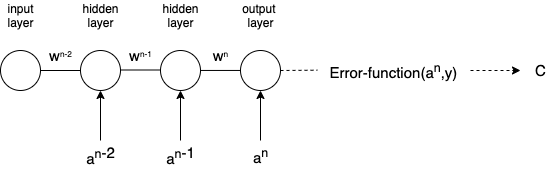
\includegraphics[scale=0.4]{latex/imgs/simplebackprop.png}
  \caption{simple neural network}\label{Baseline:before}
\end{figure}


\noindent
For a fully connected network which has more neurons per layer, the same idea can be applied. Having a neural network like the one seen in figure(14). For any neuron $i \in \{1,2,...,k\}$ in layer (n-1), and any neuron $j \in \{1,2,...,t\}$ in layer n, the impact $w_{ji}$ has on the cost is calculated by: \\

$$
\frac{\partial C}{\partial w_{ji}^n} =\frac{\partial z_j^n}{\partial w_{ji}^n}\frac{\partial a_j^n}{\partial z_j^n}\frac{\partial C}{  \partial a_j^n}
$$
Now since each neruon impact multiple neurons, which each impacts the cost, the impact of how much the activation function impacts the cost is calculated, like:

$$
\frac{\partial C}{\partial a^{n-1}_k} = \sum^t_{j=1} \frac{\partial z_j^n}{\partial a_k^{n-1}}\frac{\partial a_j^n}{\partial z_j^n}\frac{\partial C}{  \partial a_j^n}
$$

\begin{figure}[!ht]
  \centering
  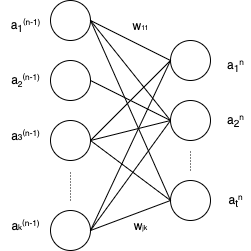
\includegraphics[scale=0.4]{latex/imgs/multibackprop.png}
  \caption{More complex neural network}\label{Baseline:before}
\end{figure}


\subsubsection{Gradient descent}
There are various of different gradient descent algorithms. As mentioned in the backpropagation section, gradient descent is a technique of measuring the degree of change w.r.t some parameter, at a certain point of a function. Gradient descent is an iteratively process that makes it path towards some local minimum. This minimum point is defined as the local minima of the function; it is not given it's the global minima. Thus, gradient descent can be applied on functions which are differentiable w.r.t it parameters. This, makes gradient descent a relatively effiecient optimization method, when looking at neural networks.\\

\noindent
There are variations of how the gradient descent is done, one of which is the Stochastic gradient descent (SGD) algorithm. When training on some dataset, usually what the programmer does is using batches, which refers to the number of samples in the dataset, which is used to calculate the gradient. Using the gradient of each individual samples results in a smoother way of finding the minima. Though, if the dataset is very big, this can quickly become a very comprehensive task. SGD relies on the random probability of randomly picking one sample from the one batch in each iteration. This means that SGD takes a single example of a gradient, instead of the sum of all gradients of the error function. As can be seen in figure(15 and 16), Doing this results in a more noisy way of finding the local minima. this doesn't matter, as long as the path it takes in finding the local minima, is actually finding the correct local minima. It's important to note, that because of the stochastic probability of picking some gradient, it is required that a lot of data is available.




\begin{figure}[h]
\centering
\begin{subfigure}{0.4\textwidth}
\centering
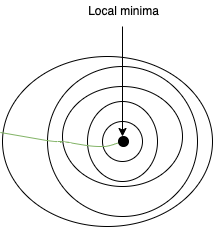
\includegraphics[scale=0.4]{latex/imgs/GDsmooth.png}
\caption{GD on each individual sample\\  in the dataset}
%\label{fig:subim1}
\end{subfigure}
\begin{subfigure}{0.4\textwidth}
\centering
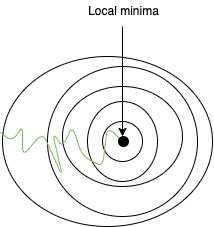
\includegraphics[scale=0.4]{latex/imgs/SGDpath.png}
\caption{SGD's path using randomly \\ selected gradient}
%\label{fig:subim2}
\end{subfigure}
\caption{Two different gradient descent paths}
\label{fig:image2}
\end{figure}

\subsubsection{Adam}
The optimizer we are using in our models is the Adam (adaptive moment estimation)  optimizer. The Adam optimizer is based on stochastic gradient descent\cite{adam}, therefor Adam has also a random probability of picking a gradient in the sample data. As well as SGD, Adam is well suited for objective functions, which require some scalar parameter maximization or minimization. \\

\noindent
Adam also uses something called gradient descent with momentum. Momentum is a method, which computes an exponentially weighted average of previously calculated gradients, and uses this gradient in the gradient descent step.

\noindent
when talking about optimizers in neural networks, "learning rate" is a keyword in this context. The learning rate is a parameter, which defines the rate of change given a gradient. This means that the greater the learning rate is, the greater the change of some specific parameter will become; in the context of finding the local minima.\\

\noindent
Adam differentiates from SGD, the way it dynamically can adjust the magnitude of how it updates the scalar parameters based on the momentum of the gradient. this means that Adam is capable of computing adaptive learning rates for different parameters\cite{adam}. Thus, for each iteration of updates in the neural network, the learning rate will be updated as well. To simplify what this means; if a gradient with respect to some parameter, has not changed for a few iterations, the learning rate for that specific gradient will be decreased.


\section{Hypothesis}

\section{Data}
In this paper we have used three different datasets, for three different purposes. The first dataset is a large dataset containing only the primary structures of proteins, which we use to train our models. The second and third datasets are significantly smaller, consisting also of the primary structures of proteins, and are labelled with structural class, and a value representing the stability of the protein respectively. The dataset containing the structural class is used as out validation set. It was never used for training, so it could be used to estimate the performance of the models. The stability dataset is used as a test set.

\subsection{Training data}
As previously mentioned, we mainly focused on the training of our models with unsupervised learning. There is a lot more data explaining the primary structure of the protein, since this is historically very easy to find, compared to finding secondary structure. \\

\noindent
Since we wanted to replicate the work of UniRep, we also chose to use UniRef50 as our training dataset.\cite{uniref} This dataset contains the primary structures of roughly \~ 27 million proteins. Due to hardware contstraints, we have decided to randomly sample 100,000 sequences from the same dataset, and use this as our training data. \\
Since we do not know how the data has been generated, we chose to randomly sample from the data, instead of taking 100k adjacent samples. We did this to avoid any kind of bias the data could have. For example, the first 100k rows of the dataset could potentially only contain one kind, or simpler and easier to process proteins. This could have an effect on the networks performance, which we have hopefully.\\

\noindent
UniRep removed proteins containing amino acid symbols (X, B, Z, J), and sequences longer than 2,000 amino acids.\cite{unirep} In our case, due to limited hardware and computer power, we chose to remove all sequences longer than 500 amino acids, and sequences containing the (X, B, Z, J) amino acids as well. The sequences containing (X, B, Z, J) are removed because they are considered "non-canonical", meaning that some of them are placeholders etc.\\

\noindent
With the sample reduction, we ended up having roughly 78,000 protein sequences in our training set. We realise that only looking at sequences with a maximum length of $500$ means that we have potentially introduced some bias into the network. This bias may make itself visible when predicting on longer proteins, where the model may think that the sequence has to end at around 500 amino acids. We argue that, in our case at least, this tradeoff is worth it because training is significantly faster, especially for the LSTM.\\

\noindent
The primary structure consists of amino acids. Each amino acid is represented as a char \\ $\in \{A, C, D, E, F, G, H, I, K, L, M, N, O, P, Q, R, S, T, U, V, W, Y\}$. Meaning that each protein from the dataset is represented as a sequence of chars, with arbitrary length. Since the length of each sequence varies, we've added a padding element (padding element is '-'); padding this element on all sequences, resulting in all sequences has a 500 feature-length. Figure ~\ref{fig:before}, shows the frequency of each amino acid in the whole dataset.\\

\begin{figure}[!ht]
  \centering
  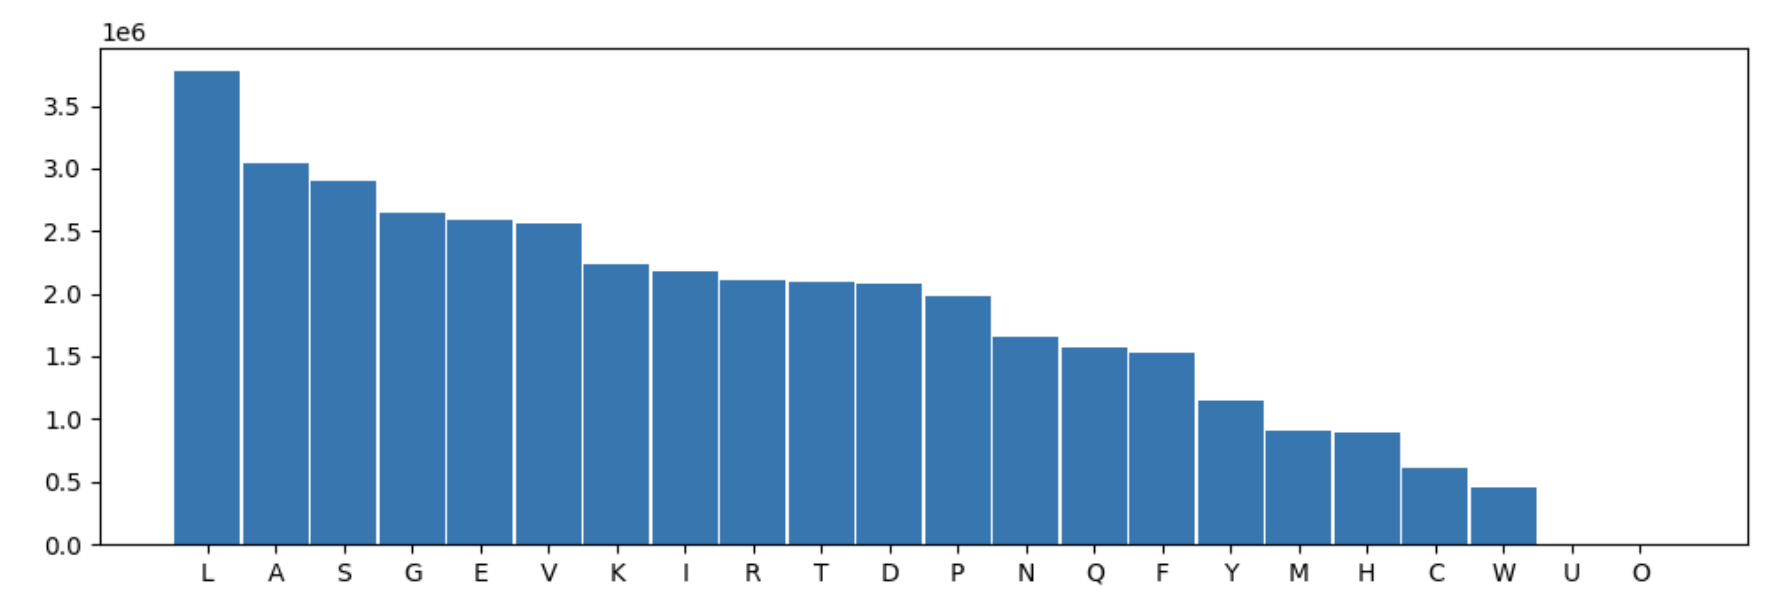
\includegraphics[scale=0.4]{latex/imgs/aminoFreq.png}
  \caption{Histogram of amino acid frequency}\label{fig:before}
\end{figure}

\noindent
Our models use embeddings, which is a method of converting a list of one-hot indices, to corresponding word embeddings. In our case, this meant that we had to transform our sequences into one-hot indices. A one-hot encoding is a way to represent the data, through a vector representation only containing \{0,1\}. Say each protein sequence only contain three amino acids (A, C, D), these amino acids will have the following one-hot encodings.

$$
A = \begin{bmatrix}
1 \\
0 \\
0
\end{bmatrix},
C = \begin{bmatrix}
0 \\
1 \\
0
\end{bmatrix},
D= \begin{bmatrix}
0 \\
0 \\
1
\end{bmatrix}
$$

\noindent
If we were looking at four amino acids (A, C, D, E), the one-hot encoding would look like:

$$
A = \begin{bmatrix}
1 \\
0 \\
0 \\
0
\end{bmatrix},
C = \begin{bmatrix}
0 \\
1 \\
0 \\
0
\end{bmatrix},
D= \begin{bmatrix}
0 \\
0 \\
1 \\
0
\end{bmatrix},
E= \begin{bmatrix}
0 \\
0 \\
0 \\
1
\end{bmatrix}
$$

\noindent
We are having working with 22 amino acids and a pad-value each amino acid will be represented $1$x$23$ onehot encoding. The onehot index describes at which index the $1$ is placed. thus if we define the onehot index of any input as $h$, we get:

\begin{align}
h(A) = 0 \\
h(C) = 1 \\
h(D) = 2 \\
h(E) = 3
\end{align}

\noindent
This means our data gets transformed to one-hot indices before we can use it in our models.

\subsection{Labelled test sets}
Since our models' performance is not measured directly on the same kind of data that we trained on, we have two datasets to use as test sets. These datasets labelled, in contrast to the training set. The first dataset has labelling detailing the structural classification of each protein.\cite{scope} The second dataset has labels describing the stability of the given proteins.\cite{stability} Both of these datasets contain the proteins' primary structure in the same format as the training dataset.\\

\noindent
\subsubsection{Structural classification}
We do not use this dataset for quantitative performance analysis. Instead, we put the models' representation of the dataset through a TSNE dimensionality reduction to see whether the different structural classifications are clearly separated. We do also note down the next token prediction accuracy of the LSTM for this dataset, but this is not necessarily a representative parameter. The data is put in several classes, as follow:
\begin{itemize}
	\item a: Alpha proteins
	\item b: Beta proteins
	\item c: Alpha/Beta proteins
	\item d: Alpha+Beta proteins. Not used
	\item e: Multi-domain proteins
	\item f: Membrane proteins
	\item g: Small proteins
\end{itemize}

\subsection{Protein Stability data}
The stability dataset is also labelled dataset containing previously explained protein sequences. In this dataset, the label explains the stability of the protein. This label is explained with some real number value, which explains how stable some protein is. This dataset we use, to check whether or not our models have learned enough of the underlying structure of the proteins, to be used to check the stability of the protein.

% \subsection{Unlabeled data}
% \subsection{Labeled data}
% \subsection{Stability data}

\section{Models and Architecture}
\subsection{Model Selection}
Choosing the right models, can in some cases be difficult. When training a neural network, there are a lot of hyperparameters that should be taken into consideration. in the pursuit of creating the most optimal neural network, it leads to a long row of hyperparameters which should be optimized. This includes the number of hidden layers, hidden neurons per each layer, learning rate, and regularization parameters. \\

\noindent
There is no method for choosing the an optimal architecture. A good architecture depends on the task - what are the model trying to achieve. Neural networks come in different forms, and each can vary a lot from each other. Tuning these hyperparameters, by trying every single combination, trying to find the ones that yield the best result, is a too comprehensive task for most computers. \\

\noindent
in our case, we have experimented with two models, a simple bottleneck CNN, and an LSTM RNN where we are replicating the work done in unirep\cite{unirep}. During this process, we used our expertise in neural networks, in choosing the correct hyperparameters for the task.


\subsection{Unirep architecture}

\subsection{LSTM reproduction of unirep}

\subsection{CNN architecture}
\subsubsection{convolutional autoencoder}

We also experimented with a CNN model, in the structure of a convolutional autoencoder. This model introduces encoding layers that reduce the dimensionality of the input $x$, down to a smaller latent representation $z$. From the latent representation, we increase the dimensions in decoding layers, with the goal of reconstructing $\hat{x}$, which is as close to the original input $x$. By doing this, the model should learn something which captures more properties of the data - more than a linear reduction method would. \\

\noindent
We start by introducing embeddings which embeds our data from a 23 channel dimension to a 12 channel dimension. The reduction of dimensions consists of 3 encoding convolutional layers. Since the features of the data are one-dimensional, we're using one-dimensional convolutions. Each of these layers all uses the ReLU activation function, to get more reliable data. This counts for all layers in the network unless the last encoder layer. We do not use ReLU here to make $z$ as general as possible. The two first encoding layers consist of average pooling, and the last consists of one max pool - reducing the dimensions to a latent space $z$.  \\

%To avoid our bottleneck from being too steep, which would result in a lot of lost properties - we chose only our latent representation $z$ is reduced to a $4$x$latent\_dimension$, where the first index is our channel size and the $latent\_dimension$ is a predefined size.\\

\noindent
From this point, our latent representation $z$ is fed into the decoder. In the decoder, it goes through the same process, of 3 convolutional layers, in which we just increase the dimensionality back to the original size.

\noindent
In each of the convolutional layers, we use convolutions with kernel\_size=5 with stride=1, by having a kernel size 5 we increase our perceptive field, this means that each convolutional layer outputs greater amounts of amount of data since it's looking at more elements at a time. Due to the boundaries of the kernel, we use padding to avoid dimension loss.\\

\noindent
Once the the the model reconstructed the original size, we use two extra convolutions, one with kernel\_size=3 and one with kernel\_size=1, both with stride=1. We do this to ensure that the model preserves the relation between the channels, once the final dimension is reached.




\section{Experiments}
\subsection{LSTM}
\subsubsection{dropout vs. not dropout}
\subsubsection{feature size}
\subsubsection{Learning rate}
\subsubsection{minimum loss model vs last model}

\subsection{CNN}
\subsubsection{overfitting}

\section{Results}
\subsection{}

\section{Discussion}
\subsection{Discussion of experiments}
\subsection{Discussion of final model}
\subsection{General discussion}

\section{Conclusion}

\section{Potential future work}
\begin{itemize}
\item Dilated kernels for CNN
\item Bidirectional LSTM, trained similar to CNN
\item Training a TCN \cite{intro}
\item Experiment with different dropout values for 2-layer LSTM
\end{itemize}

\noindent
A potential improvement of the CNN could be working with dilated kernels. Dilated convolutional kernel, are like regular convolutional kernels, but with some spacing between the values in the kernel. Dilated kernels has proved to significantly improve performance, compared to non-dilated counterparts\cite{cp}. \\

\noindent
Another potential way of making the model learn insight of the internal structure of the proteins, is instead of introducing a bottleneck, is to introduce masking. This has proven to achieve high permance in many NLP tasks\cite{BERT}. Masking is a method, which masks some tokens from the input. This mask, could be replacing the original token with another random token or a completely different value. The goal is to predict the original vocabulary before the masking. This forces the model learn some internal representation of the sequence structure.




\bibliography{latex/references}{}
\bibliographystyle{plain}

\end{document}
